\documentclass[12pt]{article}

\usepackage{sbc-template}
\usepackage{graphicx,url}
\usepackage[utf8]{inputenc}
\usepackage[brazil]{babel}
%\usepackage[latin1]{inputenc}

     
\sloppy

\title{Avaliação de desempenho de implementação paralela do método CSEM 3D no supecomputador Santos Dumont}

\author{Mateus F. Lima de Souza\inst{1,2}, Rômulo T. Lima\inst{1,3}}

\address{  Laboratório Nacional de Computação Científica (LNCC)\\
  Getúlio Vargas Av., 333, Quitandinha Petrópolis - RJ - Brasil
\nextinstitute
  Centro Federal de Educação Tecnológica Celso Suckow da Fonseca (CEFET-FR) \\
  R. Gen. Canabarro, 485 - Maracanã, Rio de Janeiro - RJ - Brasil
\nextinstitute
Universidade Católica de Petrópolis (UCP)\\
  R. Barão do Amazonas, 124 - Centro, Petrópolis - RJ - Brasil  
  \email{\{facanha,romulotl\}@lncc.br}
}

\begin{document} 

\maketitle

\begin{abstract}
  This article show the results of a parallel execution at the supercomputer Santos Dumont, the implementation of method CSEM 3D.
\end{abstract}
     
\begin{resumo} 
  Este trabalho apresenta resultado de execução paralela no supercomputador Santos Dumont, de implementação do método CSEM 3D. Neste trabalho foram desesnvolvidos conceitos e métodos de implementação de processamento paralelo, operando com grande nível de recursos computacionais. Com isso pudemos através do experimento empirico, constatar que a operação de grande quantidade de recursos, não é um sinônimo de eficiência.
\end{resumo}

\section{Introdução}
Este trabalho tem como objetivo explorar a eficiência da paralelização no código CSEM3D, utilizando como ferramenta de paralelização o OpenMPI e como recursos computacionais foram utilizados de 1 até 384 nós computacionais. O experimento consiste na confecção de duas linhas apresentando a média de tempo de execução do código CSEM3D, uma das linhas apresentando no máximo 24 processos MPI por nó computacional, já na outra representando um máximo de 48 processos pro nó computacional.

\section{CSEM} \label{sec:firstpage}
Controlled-Source Eletromagnetic (CSEM) é um método de mapeamento geofisico empregando um monitoramento eletromagnético através de sensores remotos para mapear a resistência elétrica da superfície aquática, este método utilizado em larga escala por diversas aplicações na área mineral e de mineração(Castillo-Reyes
Octavio et al; Sheard et al.2005; Yang \& Oldenburg 2012), estudos de condutividade de cristais(Castillo-Reyes
Octavio et al; Hördt et al.1992, 2000), caracterização de armazenamento de CO2 (Castillo-Reyes
Octavio et al; Girard et al.2011), projeção de reservatório geotérmico (Castillo-Reyes
Octavio et al; Coppo et al.2016) e exploração de hidrocarboneto utilizando tecnologia embarcada (Castillo-Reyes
Octavio et al; Newman \& Alumbaugh 1997; Eidesmo et al.2002; Avdeev 2005; Constable 2006; Srnka et al.2006; Orange et al.2009; Börner 2010; Constable 2010). 
\section{Processamento Paralelo}

\section{Resultados}

\begin{figure}[ht]
\centering
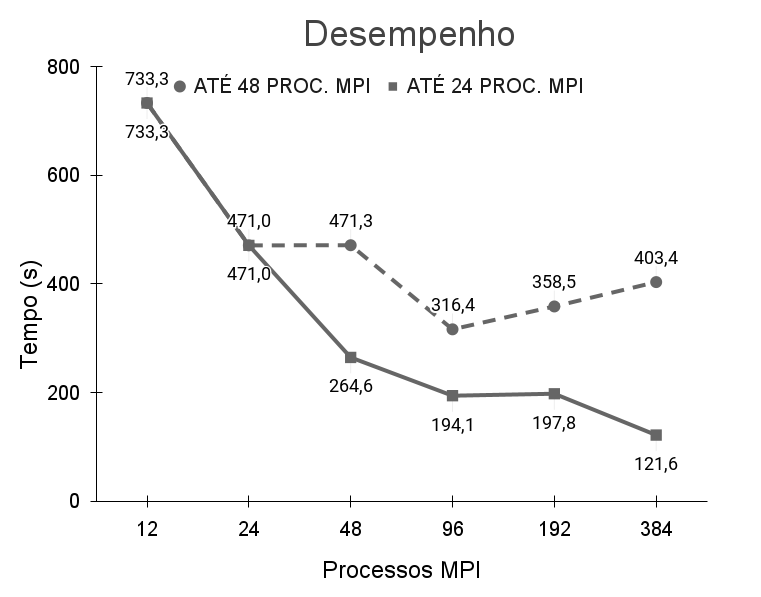
\includegraphics[width=.7\textwidth]{figures/perfpernode.png}
\caption{This figure is an example of a figure caption taking more than one line and justified considering margins mentioned in.}
\label{fig:48pernode}
\end{figure}


\section{Comentários}



Bibliographic references must be unambiguous and uniform.  We recommend giving
the author names references in brackets, e.g. \cite{knuth:84},
\cite{boulic:91}, and \cite{smith:99}.

The references must be listed using 12 point font size, with 6 points of space
before each reference. The first line of each reference should not be
indented, while the subsequent should be indented by 0.5 cm.

\bibliographystyle{sbc}
\bibliography{sbc-template}

\end{document}
